\section{Methodology}
\label{Sec3:Method}

\subsection{Preliminaries: Next-scale Prediction}
\label{subsec:preliminaries}
We formulate each video frame as a hierarchical pyramid of latent grids, adopting the structural paradigm introduced in recent scale-wise generative frameworks~\cite{tian2024visual, wang2025sampo}. Let $S$ denote the total number of spatial scales, indexed from the coarsest $s=1$ to the finest $s=S$. For a video frame at time step $t$, its multi-scale continuous latent representation is defined as:
\begin{equation}
\label{eq:pyramid_latent}
\boldsymbol{z}_t = \{\boldsymbol{z}_t^{s}\}_{s=1}^{S}, \;\; \boldsymbol{z}_t^{s} \in \mathbb{R}^{H_s \times W_s \times C_s}
\end{equation}
where $\boldsymbol{z}_t^{s}$ denotes the latent grid at scale $s$, with $(H_s, W_s)$ and $C_s$ denoting the spatial resolution and channel dimension, respectively. Unlike traditional autoregressive approaches~\cite{parkerholder2024genie2,wu2024ivideogpt,wu2024controlmllm} that flatten spatial features into a 1D raster-scan sequence, this representation inherently preserves the 2D spatial topology at each scale.

Next-scale Prediction factorizes intra-frame generation across the scale hierarchy~\cite{tian2024visual}. Given a conditioning signal $\boldsymbol{h}_t$, which encapsulates the temporal context and control inputs, the joint distribution of the latent pyramid is factorized as:
\begin{equation}
\label{eq:nextscale_factorization}
p(\boldsymbol{z}_t \mid \boldsymbol{h}_t) = \prod_{s=1}^{S} p(\boldsymbol{z}_t^{s} \mid \boldsymbol{z}_t^{<s}, \boldsymbol{h}_t), \;\; \boldsymbol{z}_t^{<s} \triangleq \{\boldsymbol{z}_t^{k}\}_{k=1}^{s-1}.
\end{equation}
where $\boldsymbol{z}_t^{<s}$ represents the collection of all coarser scales. Eq.~\eqref{eq:nextscale_factorization} implies that each feature map $\boldsymbol{z}_t^{s}$ is generated holistically conditioned on its preceding coarser structural priors $\boldsymbol{z}_t^{<s}$ and the historical context $\boldsymbol{h}_t$.
Consequently, it circumvents lengthy token-level dependencies, allowing for the integration of highly parallelizable continuous transport models.

In  action-conditioned world modeling, the conditioning variable $\boldsymbol{h}_t$ summarizes the causal dynamics up to the current state. We formalize this temporal dependency as:
\begin{equation}
\label{eq:temporal_context_def}
\boldsymbol{h}_t = \Phi(\boldsymbol{z}_{<t}, \boldsymbol{a}_{<t}), \;\; \boldsymbol{z}_{<t} \triangleq \{\boldsymbol{z}_\tau\}_{\tau < t},
\end{equation}
where $\boldsymbol{z}_{<t}$ denotes the past latent trajectory, $\boldsymbol{a}_{<t}$ indicates the sequence of executed actions, and $\Phi(\cdot)$ represents a causal temporal mapping (\textit{e.g.}, a decoder-only Transformer). Under this mathematical framework, next-scale prediction functions as a versatile interface, seamlessly linking temporal causality with continuous intra-frame synthesis.


\subsection{Problem Statement}
\label{subsec:problem_statement}
We focus on the problem of learning an action-conditioned world model to enable interactive environment simulation. Formally, the environment is modeled as a Partially Observable Markov Decision Process (POMDP), characterized by the tuple $\mathcal{M}=(\mathcal{S}, \mathcal{O}, \mathcal{A}, \mathcal{T}, \mathcal{R}, \gamma)$. At each time step $t$, the agent perceives a partial observation $\boldsymbol{o}_t \in \mathcal{O}$, executes an action $\boldsymbol{a}_t \in \mathcal{A}$, and receives a corresponding reward $r_t = \mathcal{R}(\boldsymbol{s}_t, \boldsymbol{a}_t)$ based on the unobserved true state $\boldsymbol{s}_t \in \mathcal{S}$. The core capability of a world model lies in approximating these underlying transition dynamics to support downstream planning and policy optimization. Specifically, we seek to model the joint distribution over future trajectories, conditioned on historical observations and a sequence of candidate actions:
\begin{equation}
\label{eq:wm_goal}
p(\boldsymbol{o}_{t+1:t+H}, r_{t+1:t+H} \mid \boldsymbol{o}_{1:t}, \boldsymbol{a}_{1:t+H}),
\end{equation}
where $H$ denotes the prediction horizon. 

To ensure scalability while maintaining high visual fidelity, we operate within the continuous latent space defined in Sec.~\ref{subsec:preliminaries}. Let $\boldsymbol{z}_t = \mathcal{E}(\boldsymbol{o}_t)$ denote the latent pyramid extracted by a continuous encoder $\mathcal{E}$ (following the structure in Eq.~\eqref{eq:pyramid_latent}), and let $\hat{\boldsymbol{o}}_t = \mathcal{D}(\boldsymbol{z}_t)$ represent the reconstructed observation. Consequently, our objective is to learn a parametric model $p_\theta$ that generates the future latent trajectory given a context of length $T_c$ and an action plan $\boldsymbol{a}_{1:T}$:
\begin{equation}
\label{eq:rollout_obj_latent}
p_\theta(\boldsymbol{z}_{T_c+1:T}, r_{T_c+1:T} \mid \boldsymbol{z}_{1:T_c}, \boldsymbol{a}_{1:T}).
\end{equation}
This formulation enables the agent to perform interactive rollouts and evaluate candidate action sequences to optimize decision-making. The proposed unified framework, which realizes this objective through scale-wise flow matching, is presented in Section~\ref{Sec3:UnifiedFramework}.

%%%%%%%%%%%%%%%%%%%%%%%%%%%%%%%%%%%%%%%%%%%%%%%%%%%%%%%%%%%%%%%%%%%%%%%%%%%%%%%%%%%%  
\begin{figure*}
    \centering
    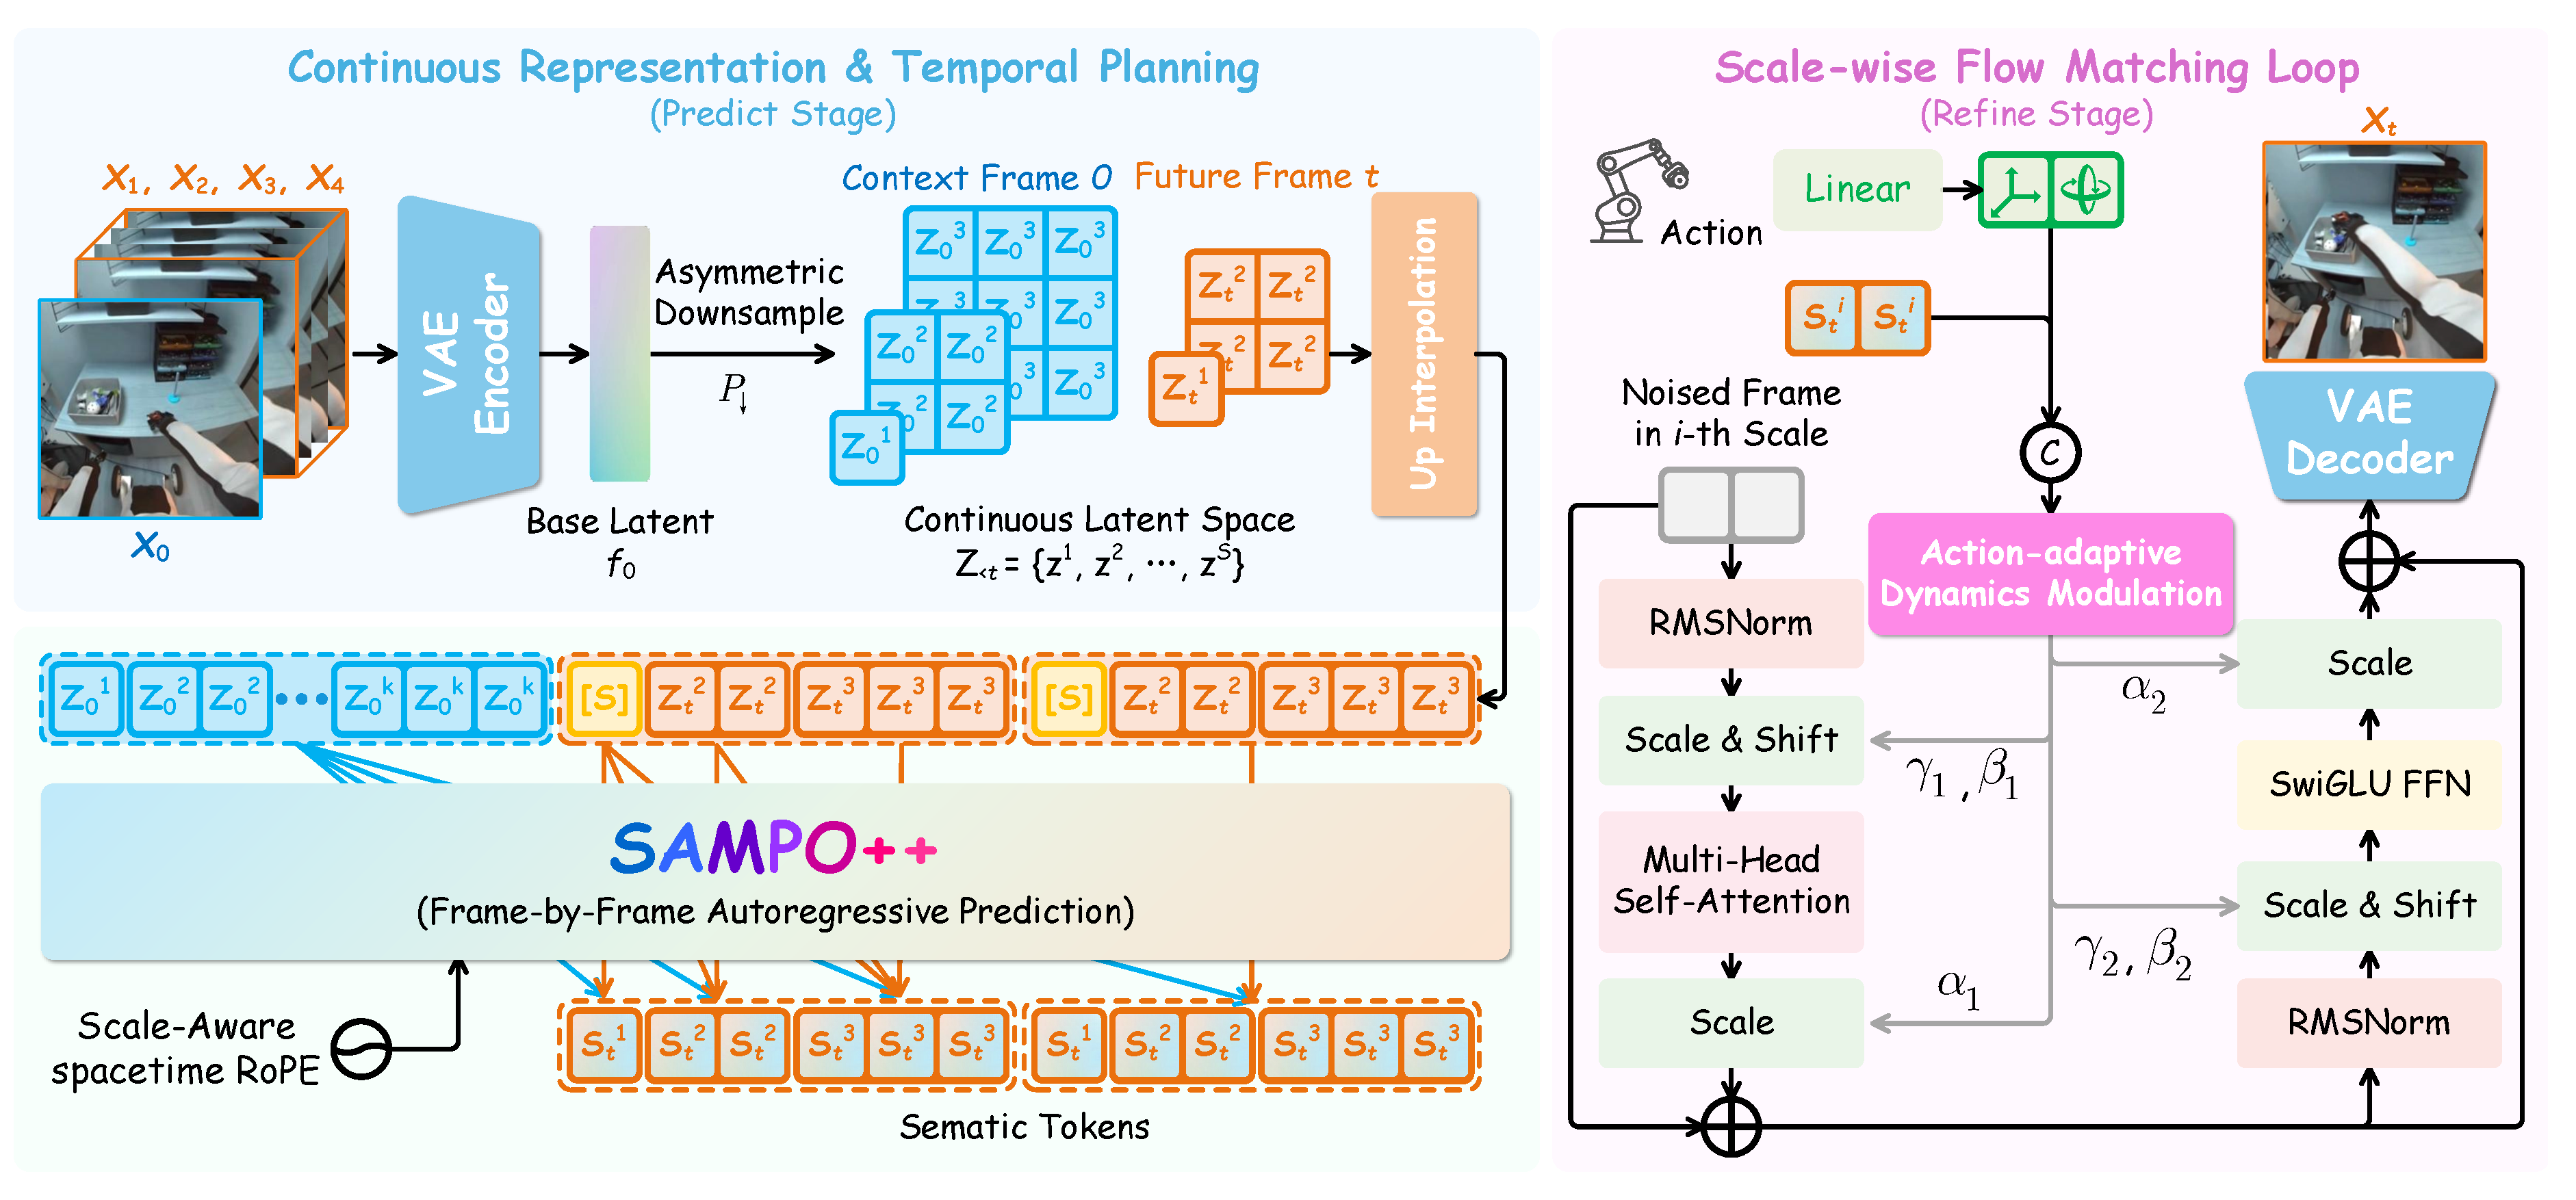
\includegraphics[width=\linewidth]{fig/fig2.pdf}
    \caption{\textbf{SAMPO++ overview}. 
    \textbf{A. Predict Stage:} Both historical context and target future frames are encoded into continuous latent pyramids via a pre-trained VAE followed by asymmetric downsampling. An autoregressive temporal planner aggregates historical features to generate multi-scale semantic representations $\{S^1, S^2, \dots\}$.
    \textbf{B. Refine Stage:} At each scale, a conditional flow matching network (parameterized as a Scale-aware DiT) predicts the velocity field required to transport noise to the target data distribution at a random timestep $t$ (timestep conditioning is omitted for simplicity). This generation process is explicitly conditioned on the semantic representations and control signals via the Action-adaptive Modulation (ADM) mechanism.}
    \label{fig2:pipline}
    % \vspace{-2ex}
\end{figure*}
%%%%%%%%%%%%%%%%%%%%%%%%%%%%%%%%%%%%%%%%%%%%%%%%%%%%%%%%%%%%%%%%%%%%%%%%%%%%%%%%%%%%  


\subsection{Continuous Pyramidal Latent Representation}
\label{Sec3:Representation}
To enable high-fidelity video generation capable of capturing subtle dynamic variations, such as fluid turbulence and lighting gradients, we fundamentally depart from the discrete tokenization paradigm prevalent in prior autoregressive world models~\cite{esser2021taming,wang2025sampo}. Although discrete codebooks facilitate categorical distribution modeling, they impose a non-differentiable quantization bottleneck. This bottleneck inherently limits the upper bound of reconstructive quality and induces high-frequency flickering artifacts~\cite{yu2023language}.

To circumvent this, we construct a continuous pyramidal latent representation to map visual observations onto a smooth, hierarchical, and differentiable manifold. 
Let $\boldsymbol{x}_t \in \mathbb{R}^{H \times W \times 3}$ denote the raw video frame at time step $t$. Rather than relying on off-the-shelf image encoders, we adopt the Vision foundation model Aligned Variational AutoEncoder (VA-VAE) framework~\cite{yao2025reconstruction}. By leveraging rigorous in-domain pre-training, we explicitly align the empirical visual distribution with our continuous manifold. This domain-aligned encoder $\mathcal{E}$ is subsequently deployed to extract a robust base latent feature map $\boldsymbol{f}_t^0 \in \mathbb{R}^{h \times w \times c}$. 
Crucially, we bypass the quantization operation entirely, retaining the continuous latent distributions parameterized by their moments for downstream modeling.

To establish the multi-scale hierarchy required for coarse-to-fine generation, we introduce a recursive downsampling operator $\mathcal{P}_{\downarrow}$, inspired by Laplacian pyramids~\cite{denton2015deep}. The resulting latent pyramid $\mathcal{Z}_t = \{ \boldsymbol{z}_t^1, \boldsymbol{z}_t^2, \dots, \boldsymbol{z}_t^S \}$ is defined as:
\begin{equation}
    \boldsymbol{z}_t^S = \boldsymbol{f}_t^0, \;\; \boldsymbol{z}_t^{s-1} = \mathcal{P}_{\downarrow}(\boldsymbol{z}_t^s), \;\; \text{for } s = S, \dots, 2,
\end{equation}
where $S$ denotes the total number of scales. The scale $s=S$ corresponds to the finest resolution containing intricate texture details, while $s=1$ represents the coarsest resolution (\textit{e.g.}, $1 \times 1$ or $2 \times 2$) describing the global semantic layout. Mathematically, the feature map at scale $s$ lies in the space $\mathbb{R}^{h_s \times w_s \times c}$, where $h_s = h / 2^{S-s}$ and $w_s = w / 2^{S-s}$.

Adopting this continuous framework yields two significant theoretical advantages over discrete tokenization. First, it inherently preserves manifold continuity. By operating within $\mathbb{R}^n$, the representation space remains unfragmented, which allows the generative model to approximate the true data distribution with arbitrary precision. This effectively avoids the quantization error inherent in discrete approaches, wherein the true latent state falls between two codebook centroids. Second, it ensures compatibility with gradient-based dynamics. Continuous vectors naturally align with the Ordinary Differential Equation (ODE) framework utilized in Flow Matching~\cite{chen2018neural, lipman2023flow}. This alignment enables us to model the transition between scales as a smooth trajectory integration problem, in stark contrast to the categorical classification tasks required by discrete tokenization.

\subsection{Unified Temporal Autoregressive with Scale-wise Flow Matching}
\label{Sec3:UnifiedFramework}
The core premise of SAMPO++ lies in disentangling the complexity of world modeling into two orthogonal axes: Time and Resolution. We observe that relying solely on autoregression~\cite{esser2021taming,wu2024ivideogpt,brown2020language,yan2021videogpt} is computationally prohibitive for high-dimensional visual data. Conversely, relying exclusively on diffusion or flow models~\cite{blattmann2023stable,zhu2024sora,lipman2023flow,dao2023flow} fails to capture the explicit causal reasoning required for effective planning.
To bridge this gap, we introduce a hybrid probabilistic framework that decomposes the joint distribution $p(\boldsymbol{z}_{1:T})$ into an Inter-frame Temporal Autoregressive component responsible for causal planning, and an Intra-frame Scale-wise Flow component dedicated to high-fidelity rendering. This architecture embodies a "Predict-then-Refine" paradigm, which is mathematically formulated as:
\begin{equation}
    p_\theta(\boldsymbol{z}_{1:T} | \boldsymbol{a}_{1:T}) = \prod_{t=1}^{T} \underbrace{p_\theta(\boldsymbol{h}_t | \boldsymbol{z}_{<t}, \boldsymbol{a}_{<t})}_{\text{Inter-frame Planning}} \cdot \prod_{s=1}^{S} \underbrace{p_\theta(\boldsymbol{z}_t^s | \boldsymbol{z}_t^{<s}, \boldsymbol{h}_t)}_{\text{Intra-frame Refinement}}.
\end{equation}
The following subsections elaborate on these components and their synergistic integration.

\noindent \textit{\textbf{1) Inter-frame Temporal Autoregression: The Causal Planner.}}
The fundamental objective of the temporal module is to model the causal evolution of the environment's state dynamics. Rather than predicting raw pixels or stochastic high-frequency details, which are inherently intractable to model autoregressively~\cite{van2016pixel, yan2021videogpt}, this module is dedicated to inferring a Temporal Context Vector $\boldsymbol{h}_t$. This vector acts as a structural prior, encapsulating both the deterministic physics and the semantic intent governing the subsequent frame.

As illustrated in the predict stage of Figure~\ref{fig2:pipline}, we instantiate this module utilizing a scalable causal transformer backbone~\cite{tian2024visual}, denoted as $\mathcal{T}_{\text{time}}$. This network is composed of stacked decoder-only transformer blocks and operates strictly on the sequence of historical finest-scale latents. Defining the history horizon as $\mathcal{H}_{<t} = \{ (\boldsymbol{z}_{1}^S, \boldsymbol{a}_{1}), \dots, (\boldsymbol{z}_{t-1}^S, \boldsymbol{a}_{t-1}) \}$, the temporal forward pass is formulated as:
\begin{equation}
    \boldsymbol{h}_t = \mathcal{T}_{\text{time}}(\text{Embed}(\mathcal{H}_{<t}); \theta_{\text{AR}}),
\end{equation}
where $\boldsymbol{h}_t \in \mathbb{R}^{D}$ is a dense vector acting as a global structural prior for time step $t$.

Crucially, this formulation distinguishes our approach from standard video transformers~\cite{yan2021videogpt, rakhimov2020latent} in two key aspects. First, regarding latent-space operation, the planner processes the highly compressed continuous latent space $\boldsymbol{z}^S$ instead of raw pixels. This design effectively reduces the spatial sequence length by orders of magnitude, thereby enabling computationally efficient long-horizon reasoning—a strategy validated in latent diffusion frameworks~\cite{rombach2022high}. Second, concerning the role of conditioning, the output $\boldsymbol{h}_t$ serves not as the generated frame itself but as an abstract condition for the subsequent generative flow. By relieving the autoregressive module from the burden of synthesizing high-frequency noise, we allow the planner to focus strictly on maintaining temporal consistency and object permanence.

\noindent \textit{\textbf{2) Intra-frame Scale-wise Flow: The Continuous Renderer.}}
Guided by the temporal plan $\boldsymbol{h}_t$ and the coarser structural priors $\boldsymbol{z}_t^{<s}$, the objective of the Intra-frame module is to synthesize the detailed feature map $\boldsymbol{z}_t^s$ at the current scale $s$. We leverage Conditional Flow Matching (CFM), a simulation-free approach for training Continuous Normalizing Flows (CNFs)~\cite{lipman2023flow, albergo2025stochastic, dao2023flow}, to model the complex transition from a tractable noise distribution to the data distribution.

We ground our generative modeling in the framework of probability flow Ordinary Differential Equations (ODEs). Specifically, we define a time-dependent probability density path $p_\tau(\boldsymbol{x})$, where $\tau \in [0, 1]$ denotes the flow time, a variable distinct from the video timestamp $t$. The generation process entails solving an ODE that integrates from Gaussian noise $\boldsymbol{x}_0 \sim \mathcal{N}(\boldsymbol{0}, \boldsymbol{I})$ to the target data sample $\boldsymbol{x}_1 = \boldsymbol{z}_t^s$:
\begin{equation}
    d\boldsymbol{x}_\tau = v_\theta(\boldsymbol{x}_\tau, \tau; \text{cond}_{t,s}) \, d\tau,
\end{equation}
where $v_\theta$ represents a neural velocity field parameterized by a Diffusion Transformer~\cite{peebles2023scalable, yao2025reconstruction}, and $\text{cond}_{t,s} = \{ \boldsymbol{z}_t^{<s}, \boldsymbol{h}_t \}$ denotes the composite conditioning signal.

To facilitate efficient and stable sampling, we supervise this model by enforcing an Optimal Transport (OT) conditional vector field~\cite{lipman2023flow}. By minimizing transport cost, this method establishes straight-line trajectories between the noise distribution and the data distribution~\cite{liuflow}. The target vector field is defined as $u_\tau(\boldsymbol{x}|\boldsymbol{x}_1, \boldsymbol{x}_0) = \boldsymbol{x}_1 - \boldsymbol{x}_0$, leading to the following regression objective:
\begin{equation}
    \mathcal{L}_{\text{Flow}} = \mathbb{E}_{\tau, \boldsymbol{x}_0, \boldsymbol{x}_1} \left[ || v_\theta(\psi_\tau(\boldsymbol{x}_0, \boldsymbol{x}_1), \tau; \text{cond}_{t,s}) - (\boldsymbol{x}_1 - \boldsymbol{x}_0) ||^2 \right],
\end{equation}
where $\psi_\tau(\boldsymbol{x}_0, \boldsymbol{x}_1) = (1-\tau)\boldsymbol{x}_0 + \tau\boldsymbol{x}_1$ represents the linear interpolation state.
To instantiate the velocity field $v_\theta$, we augment the DiT block by replacing LayerNorm with RMSNorm and applying 2D RoPE in all attention layers~\cite{yao2025reconstruction}. Within this augmented architecture, we employ a highly effective dual-injection strategy to incorporate the multi-source conditions. First, for spatial and contextual guidance, the coarser latent $\boldsymbol{z}_t^{<s}$ and the temporal plan $\boldsymbol{h}_t$ are upsampled (if necessary) and strictly concatenated with the noisy state $\boldsymbol{x}_\tau$ along the channel dimension, thereby bounding the velocity field within the established structural envelope. Second, to enforce precise controllability, the action signal $\boldsymbol{a}_t$ is actively injected into the intermediate features via our proposed Action-adaptive Dynamics Modulation (ADM) mechanism. This unified architectural choice ensures that the generated microscopic details, including motion blur and subtle lighting variations, remain strictly coherent with the macroscopic physical evolution predicted by the temporal planner.

By recursively applying this optimal transport process from scale $s=1$ to $S$, SAMPO++ synthesizes high-fidelity frames that are simultaneously physically grounded (governed by $\boldsymbol{h}_t$ and $\boldsymbol{a}_t$) and structurally coherent (guided by $\boldsymbol{z}_t^{<s}$).

\begin{figure}
    \centering
    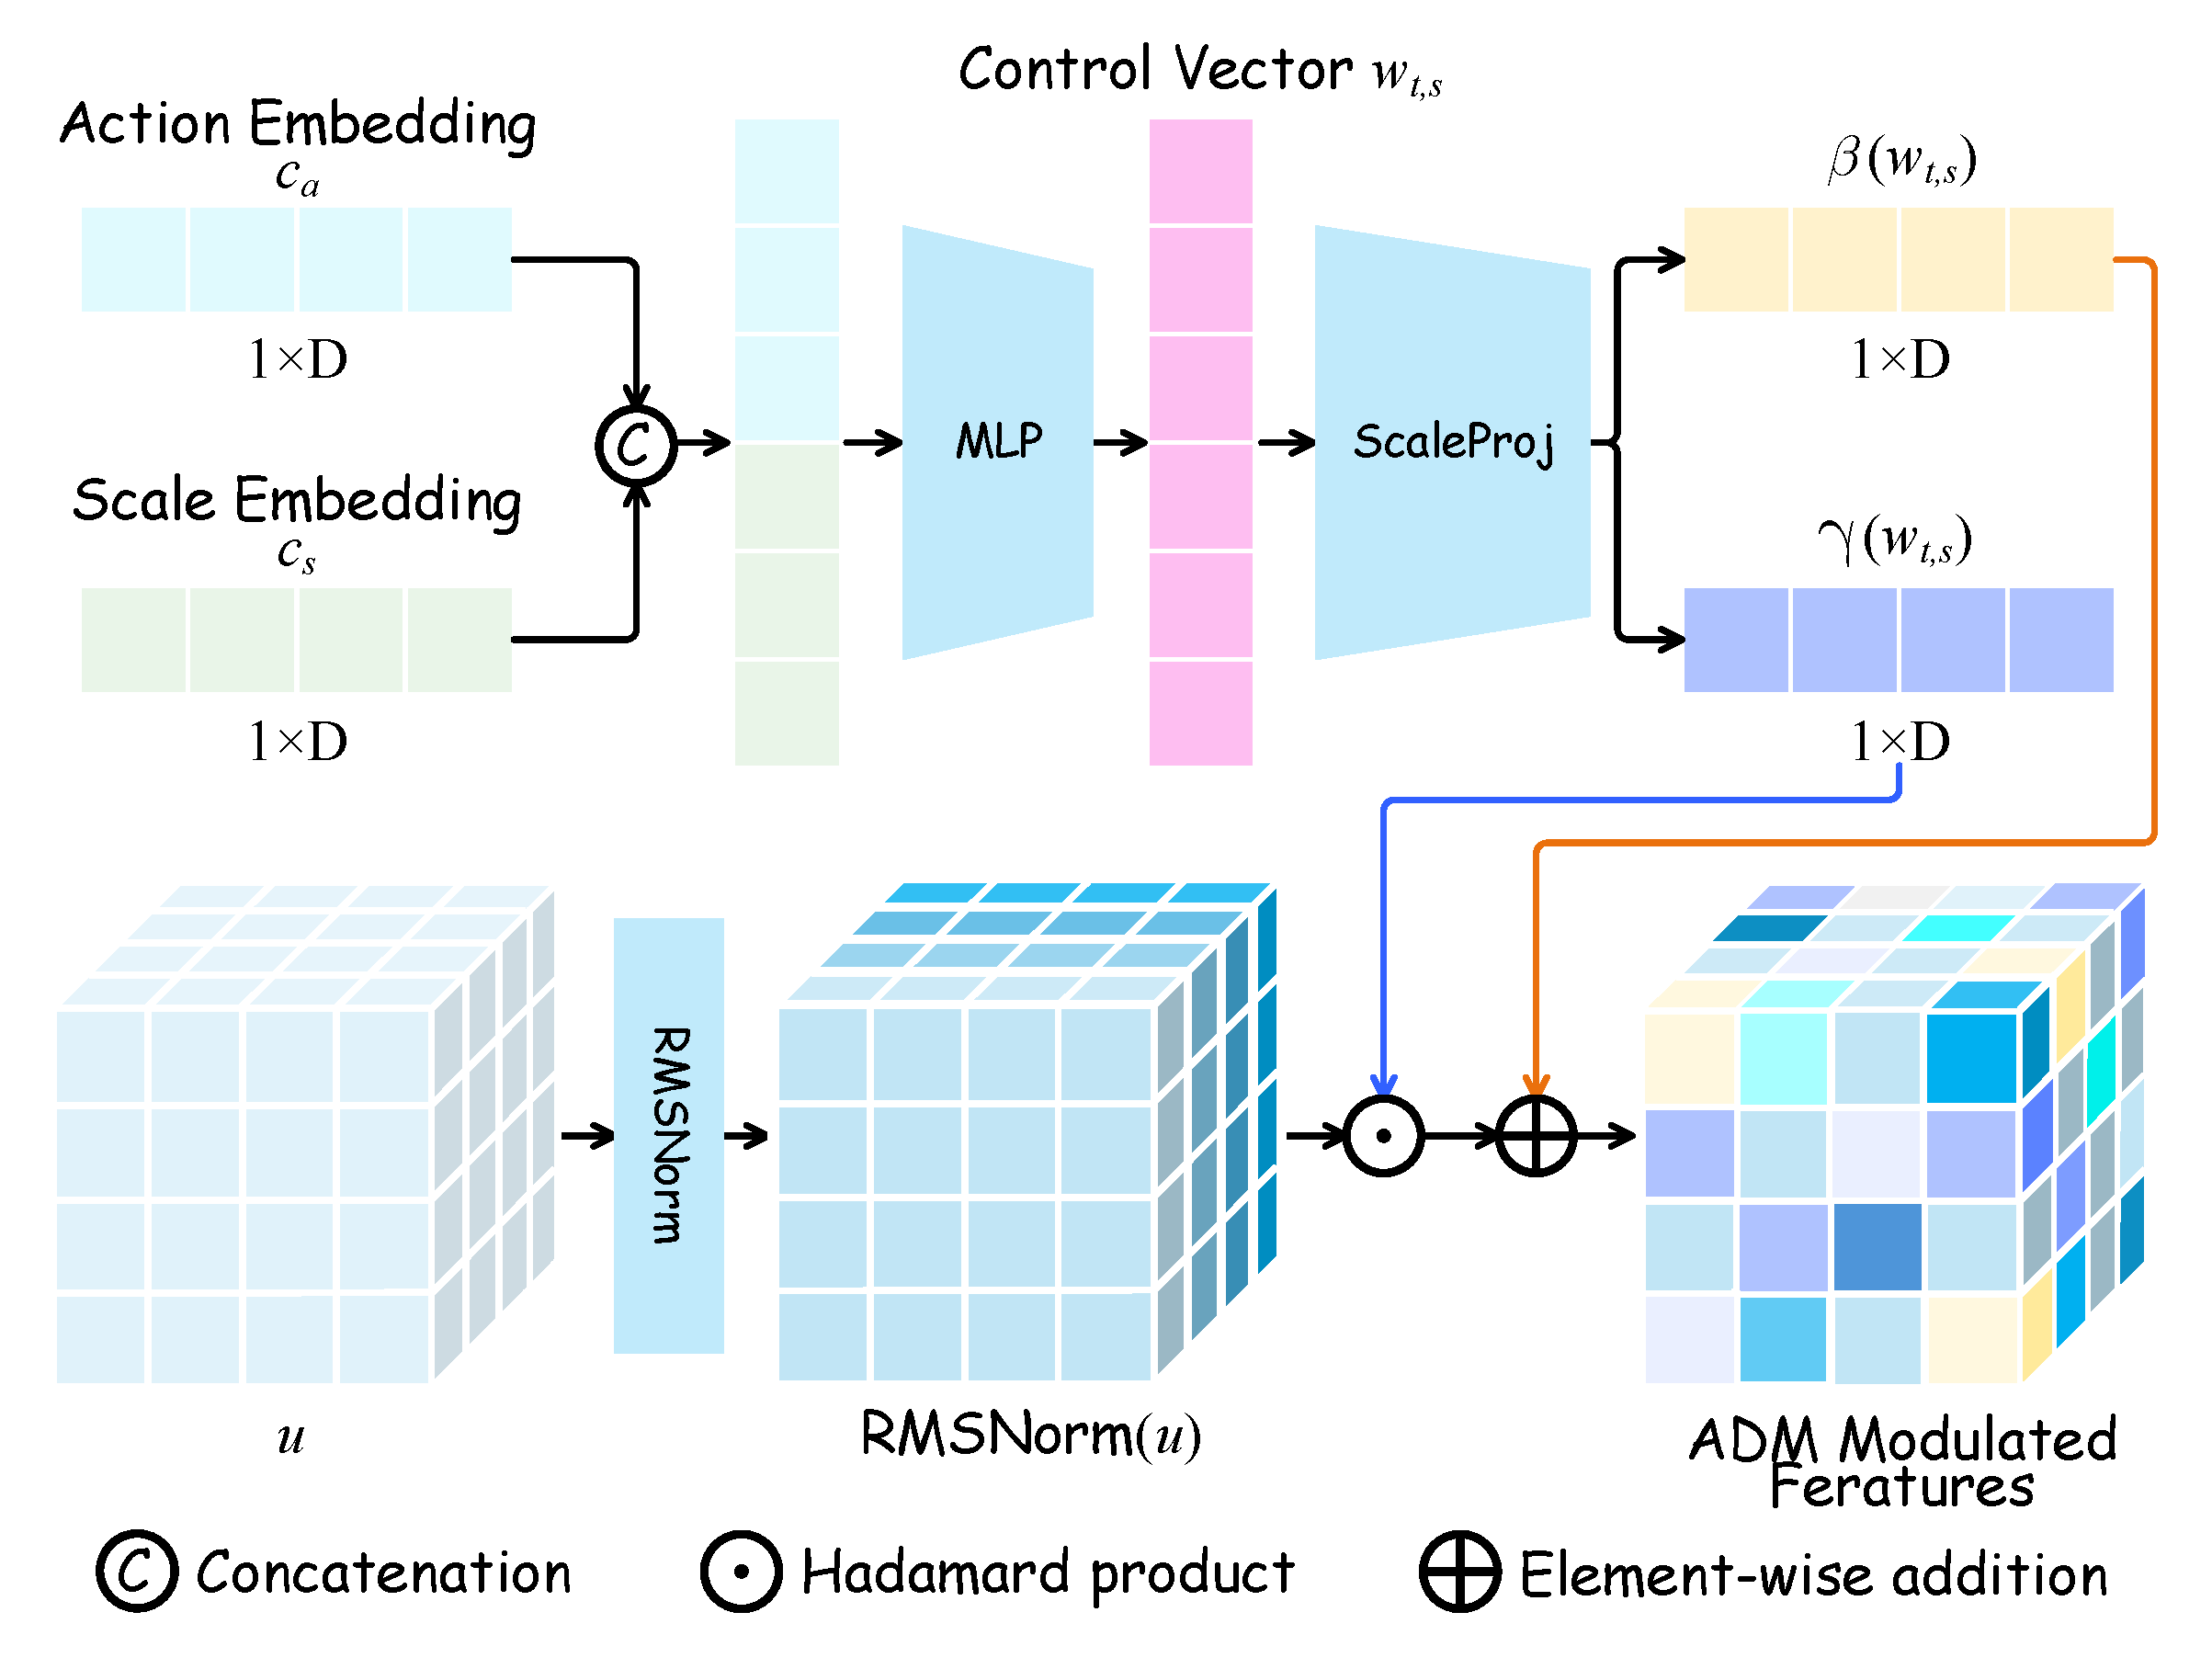
\includegraphics[width=1.0\linewidth]{fig/fig_ADM.pdf}
    \caption{\textbf{Action-adaptive Dynamics Modulation (ADM).} ADM explicitly alters the generative dynamics by modulating intermediate feature statistics. It fuses action and scale embeddings to regress affine parameters ($\boldsymbol{\gamma}$, $\boldsymbol{\beta}$).}
    \label{fig:fig_ADM}
    \vspace{-1ex}
\end{figure}

\subsection{Action-adaptive Dynamics Modulation}
\label{Sec3:ActionModulation}
Existing approaches typically treat actions $\boldsymbol{a}_t$ merely as passive tokens via concatenation or cross-attention~\cite{mou2024t2i, wang2025sampo}. This passive injection is inadequate for physics-based simulation because it fails to explicitly modulate the underlying generative vector field. Furthermore, these signals easily attenuate across deep layers, exacerbating the severe ``action forgetting'' phenomenon.

In response, we propose Action-adaptive Dynamics Modulation (ADM), as illustrated in Figure~\ref{fig:fig_ADM}. This mechanism systematically integrates adaptive normalization principles~\cite{karras2019stylegan2, park2019semantic, yu2025pixeldit} into the flow matching paradigm. Our core insight is that actions should function as global system parameters that actively and directly modulate the intermediate feature statistics of the network. Crucially, we posit that this modulation must be intrinsically scale-aware: microscopic actions (\textit{e.g.}, ``gripper close'') induce localized, high-frequency deformations, whereas macroscopic actions (\textit{e.g.}, ``move forward'') govern low-frequency global displacements. 

We embed ADM directly within the augmented Transformer blocks~\cite{yao2025reconstruction} of our Flow Matching network. For a specific architectural scale $s$ and timestep $t$, we first synthesize a scale-aware control vector $\boldsymbol{w}_{t,s}$ by fusing the time-dependent action embedding $\boldsymbol{c}_a$ with a learnable scale embedding $\boldsymbol{c}_s$:
\begin{equation}
    \boldsymbol{w}_{t,s} = \text{MLP}([ \boldsymbol{c}_a, \boldsymbol{c}_s ]),
\end{equation}
where $[\cdot, \cdot]$ denotes channel-wise concatenation. This intermediate representation is subsequently projected to regress the scale and shift parameters, $\boldsymbol{\gamma}$ and $\boldsymbol{\beta}$, for affine transformation:
\begin{equation}
    \boldsymbol{\gamma}(\boldsymbol{w}_{t,s}), \boldsymbol{\beta}(\boldsymbol{w}_{t,s}) = \text{ScaleProj}(\boldsymbol{w}_{t,s}).
\end{equation}

Within each Transformer block, this active modulation is applied to the intermediate latent feature representation $\boldsymbol{u}$ prior to the self-attention and Feed-Forward Network (FFN) modules. Consistent with our architectural modifications detailed in Section~\ref{Sec3:UnifiedFramework}, we employ RMSNorm to stabilize the continuous flow integration:
\begin{equation}
    \text{ADM}(\boldsymbol{u}, \boldsymbol{a}_t, s) = (\boldsymbol{1} + \boldsymbol{\gamma}_{t,s}) \odot \text{RMSNorm}(\boldsymbol{u}) + \boldsymbol{\beta}_{t,s}.
\end{equation}

Conceptually, this formulation establishes a more mathematically principled integration of control signals into the generation dynamics. In Flow Matching, the neural network parameterizes the velocity field of the probability flow ODE. By modulating the activation statistics via $\boldsymbol{\gamma}$ and $\boldsymbol{\beta}$, ADM continuously applies an action-conditioned affine transformation to the latent manifold. This topological constraint ensures that the action signal imposes a strong, persistent inductive bias along the entire generative trajectory and across all network depths, thereby effectively eradicating action forgetting and yielding superior kinematic control fidelity compared to standard passive conditioning.


\begin{figure}
    \centering
    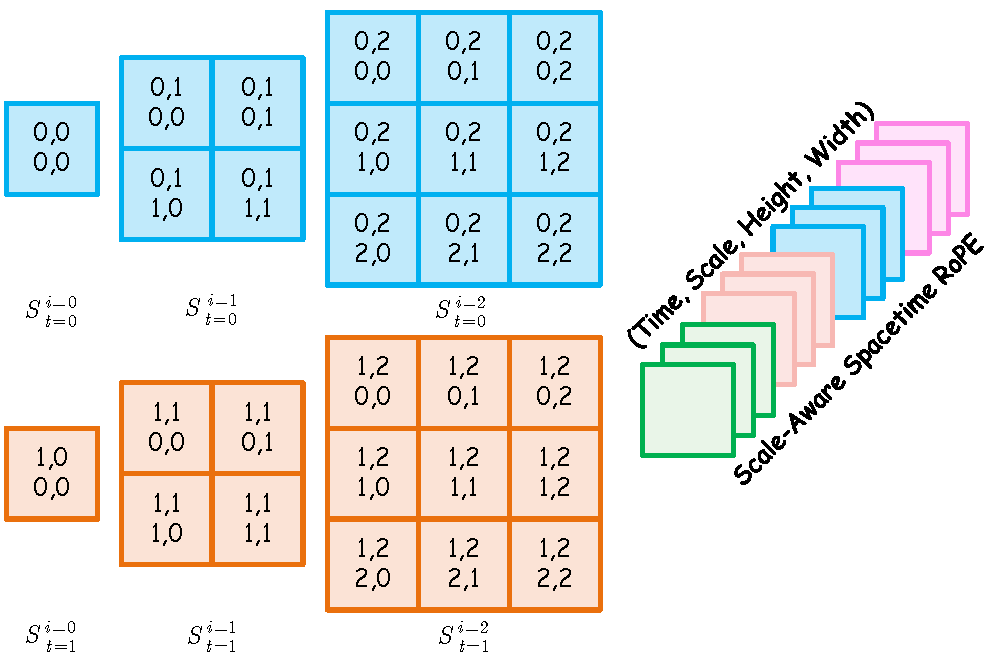
\includegraphics[width=0.95\linewidth]{fig/fig_SAROPE.pdf}
     \caption{\textbf{Scale-Aware spacetime RoPE (SA-RoPE).} To mitigate error accumulation in continuous latent spaces, SA-RoPE factorizes positional information into orthogonal rotational components across time, scale, and spatial dimensions. 
     }
    \label{fig:fig_SAROPE}
    \vspace{-1ex}
\end{figure}


\subsection{Long-horizon Spatiotemporal Consistency Enforcement}
\label{Sec3:Consistency}
Autoregressive models operating within continuous latent spaces are inherently susceptible to error accumulation~\cite{pasini2024continuous}. In this regime, minor deviations in early frames can rapidly propagate and cascade into severe structural degradation over extended horizons. In contrast to discrete representations, which implicitly rectify errors by quantizing latents to the nearest codebook centroid~\cite{van2017neural}, continuous errors can accumulate unboundedly. To mitigate this issue, we incorporate a strong structural inductive bias via SA-RoPE and an inference-time physical constraint known as Flow Rectification~\cite{liuflow}.

While standard RoPE~\cite{su2024roformer} effectively handles 1D sequences or 2D spatial grids, SAMPO++ operates on a more complex 4D manifold defined by coordinates $(t, s, h, w)$ representing time, scale, height, and width. Omitting the scale dimension in positional encoding introduces ambiguity, as the attention mechanism struggles to distinguish between structurally similar features originating from different resolution levels. To address this limitation, we formulate a Scale-Aware spacetime RoPE (SA-RoPE) that factorizes positional information into orthogonal rotational components (see Figure~\ref{fig:fig_SAROPE}). For a query vector $\boldsymbol{q}$ located at $(t, s, h, w)$, the transformed embedding is obtained via the composition of three independent rotations:
\begin{equation}
    \boldsymbol{q}' = \boldsymbol{q} \boldsymbol{R}_{\text{time}}(t) \boldsymbol{R}_{\text{scale}}(s) \boldsymbol{R}_{\text{spatial}}(h, w).
\end{equation}
The term $\boldsymbol{R}_{\text{scale}}(s)$ is critical for our scale-wise generation paradigm as it explicitly encodes the frequency level of the current feature. This enables attention heads to learn specialized behaviors, such as retrieving global structure from coarse scales ($s=1$) versus refining local textures at fine scales ($s=S$). By rigorously anchoring features within this 4D coordinate system, the model preserves superior structural coherence across long temporal windows.

\begin{algorithm}[t]
\caption{SAMPO++ Training (End-to-End)}
\label{algo:training}
\begin{algorithmic}[1]
\REQUIRE Dataset $\mathcal{D}$, Encoder $\mathcal{E}$, Causal Planner $\mathcal{T}$, FlowNet $v_\theta$, Downsample $\mathcal{P}_{\downarrow}$
\STATE $(\boldsymbol{x}, \boldsymbol{a}) \sim \mathcal{D}$; $\boldsymbol{z} = \mathcal{E}(\boldsymbol{x})$; Pyramid $\mathcal{Z} = \{\mathcal{P}_{\downarrow}(\boldsymbol{z}_t)\}_{t=1, s=1}^{T, S}$;
\STATE $\mathcal{L}_{\text{total}} = 0$;
\FOR{$t = 1, \dots, T$}
    \STATE $\hat{\boldsymbol{h}}_t = \mathcal{T}(\boldsymbol{z}_{<t}^S, \boldsymbol{a}_{<t})$; 
    \STATE $\boldsymbol{z}_t^0 = \boldsymbol{0}$; 
    \FOR{$s = 1, \dots, S$}
        \STATE $\tau \sim U(0,1), \ \boldsymbol{\epsilon} \sim \mathcal{N}(\boldsymbol{0}, \boldsymbol{I})$;
        \STATE $\boldsymbol{x}_\tau = (1-\tau)\boldsymbol{\epsilon} + \tau \boldsymbol{z}_t^s$; \ \ $\boldsymbol{c} = [ \text{up}(\boldsymbol{z}_t^{s-1}) , \hat{\boldsymbol{h}}_t ]$;
        \STATE $\boldsymbol{m} = \text{ADM}(\boldsymbol{a}_t, s)$; \ \ $\hat{\boldsymbol{v}} = v_\theta(\boldsymbol{x}_\tau, \tau, \boldsymbol{c}, \boldsymbol{m})$;
        \STATE $\mathcal{L}_{\text{Flow}} = \|\hat{\boldsymbol{v}} - (\boldsymbol{z}_t^s - \boldsymbol{\epsilon})\|_2^2$;
        \STATE $\mathcal{L}_{\text{total}} \leftarrow \mathcal{L}_{\text{total}} + w_s \cdot \mathcal{L}_{\text{Flow}}$;
    \ENDFOR
\ENDFOR
\STATE Update all parameters $(\theta_{\mathcal{T}}, \theta_{v})$ via $\nabla \mathcal{L}_{\text{total}}$;
\end{algorithmic}
\end{algorithm}
\begin{algorithm}[t]
\caption{SAMPO++ Inference}
\label{algo:inference}
\begin{algorithmic}[1]
\REQUIRE Context Frames $\boldsymbol{x}_{\text{ctx}}$, Action Plan $\boldsymbol{a}_{\text{fut}}$, Decoder $\mathcal{D}$
\STATE Initialize history buffer: $\mathcal{H} = \{ \mathcal{E}(\boldsymbol{x}_{\text{ctx}})^S \}$; 
\FOR{$k = 1, \dots, K$}
    \STATE $\hat{\boldsymbol{h}}_k = \mathcal{T}(\mathcal{H}, \boldsymbol{a}_{<k})$;
    \STATE $\boldsymbol{z}_k^0 = \boldsymbol{0}$; 
    \FOR{$s = 1, \dots, S$}
        \STATE $\boldsymbol{c} = [ \text{up}(\boldsymbol{z}_k^{s-1}), \hat{\boldsymbol{h}}_k ]$;
        \STATE $\boldsymbol{m} = \text{ADM}(\boldsymbol{a}_k, s)$; 
        \STATE $\boldsymbol{z}_k^s = \text{ODESolve}\big(\mathcal{N}(\boldsymbol{0}, \boldsymbol{I}), v_\theta(\cdot, \tau, \boldsymbol{c}, \boldsymbol{m}), \text{Rectify}\big)$; 
    \ENDFOR
    \STATE $\mathcal{H} \leftarrow \mathcal{H} \cup \{\boldsymbol{z}_k^S\}$; 
\ENDFOR
\RETURN $\hat{\boldsymbol{x}}_{\text{fut}} = \mathcal{D}(\mathcal{H}_{\text{fut}})$;
\end{algorithmic}
\end{algorithm}

Although SA-RoPE imparts structural awareness during the training phase, it does not actively mitigate latent drift during the inference process. To enforce strict physical consistency, we introduce a flow trajectory rectification strategy that operates as an energy-based guidance mechanism during sampling. We postulate that the temporal evolution of latent features must maintain consistency with the estimated optical flow. Let $\boldsymbol{F}_{t-1 \to t}$ denote the dense optical flow field predicted by a lightweight estimator, such as RAFT~\cite{teed2020raft}. We define a consistency energy function $E(\boldsymbol{z}_t^s)$ to measure the discrepancy between the generated latent and the warped state of the previous frame:
\begin{equation}
    E(\boldsymbol{z}_t^s) = \frac{1}{2} \| \boldsymbol{z}_t^s - \mathcal{W}(\boldsymbol{z}_{t-1}^s, \boldsymbol{F}_{t-1 \to t}) \|_2^2,
\end{equation}
where $\mathcal{W}$ denotes the warping operator. Given that Flow Matching generation entails solving the probability flow ODE~\cite{lipman2023flow, albergo2025stochastic}, we rectify the trajectory by augmenting the velocity field $v_\theta$ at each integration step. This is achieved by injecting the negative gradient of the consistency energy:
\begin{equation}
    v_{\text{rectified}}(\boldsymbol{z}_\tau, \tau) = v_\theta(\boldsymbol{z}_\tau, \tau) - \lambda(\tau) \nabla_{\boldsymbol{z}_\tau} E(\boldsymbol{z}_\tau),
\end{equation}
where $\lambda(\tau)$ is a time-dependent guidance scale. This operation effectively steers the generative trajectory towards physically plausible states that respect optical flow continuity equations, thereby significantly extending the stable rollout horizon without requiring retraining of the base model.

The complete training and inference procedures of SAMPO++ are summarized in Algorithm~\ref{algo:training} and Algorithm~\ref{algo:inference}, respectively. Notably, during the inference phase, we utilize the KV cache~\cite{pope2023efficiently} within the autoregressive causal planner to efficiently generate each temporal context $\boldsymbol{h}_t$ without redundant historical computation.